\subsection{Welcome}
\label{sub:Welcome}

\frnote{læs igennem}

Welcomemodulet har til opgave at lave det skærmbillede man bliver præsenteret for når man først logger ind.

\subsubsection{Implementation}
\label{ssub:Welcome_implementation}
Welcome åbnes fra styringsmoduler og står for at udfylde den tab der først vises. På dette skærmbillede skal der være nyttige funktioner for den bruger der lige er logget ind. Derudover skal der også være relevante informationer for brugeren.

\begin{figure}
  \centering
  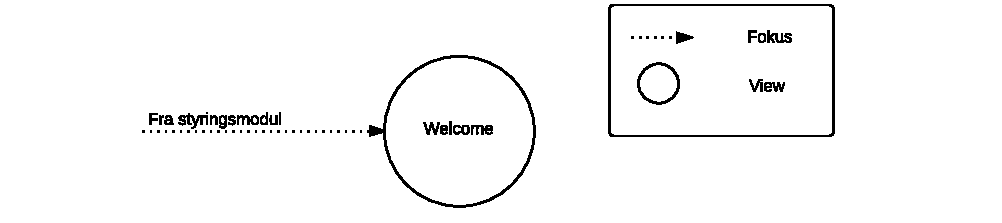
\includegraphics[width=\textwidth]{forside-diagram.pdf}
  \caption{Diagram over Welcomemodulet}
  \label{fig:forsidemod}
\end{figure}
% GuestCreatormodulet, der fremstår som \enquote{Ny Gæst} på \cref{fig:guestcreator}, består af et GuestCreator-view og en GuestController. Den data der indtastes i GuestCreator view'et, sendes videre til GuestControlleren. Herefter kommunikerer GuestCotrolleren med persistenslaget, som derefter gemmer informationen om den nye gæst.